\documentclass{article}
\usepackage{tikz}
\usepackage[a4paper]{geometry}
\usepackage{fancyhdr}
\pagestyle{fancy}
\lhead{Kladogramme}
\rhead{März 2026}
\begin{document}
\section{Kladogramme}
\subsection{Kladogramme}
\emph{Kladogramme} stellen die Evolution der Arten dar.
 
Auf einem Zeitstrahl wird eine Linie welche von der einen Art, über die Artenbildung, sich in zwei teilend, bis zu den zwei neuen Arten. Auf den einzelnen Segmenten der Linie sind Punkte mit zurzeitigen Merkmalen der Arten. Im besten Falle sind Jahreszahlen bekannt und angegeben.
 
\begin{center}
 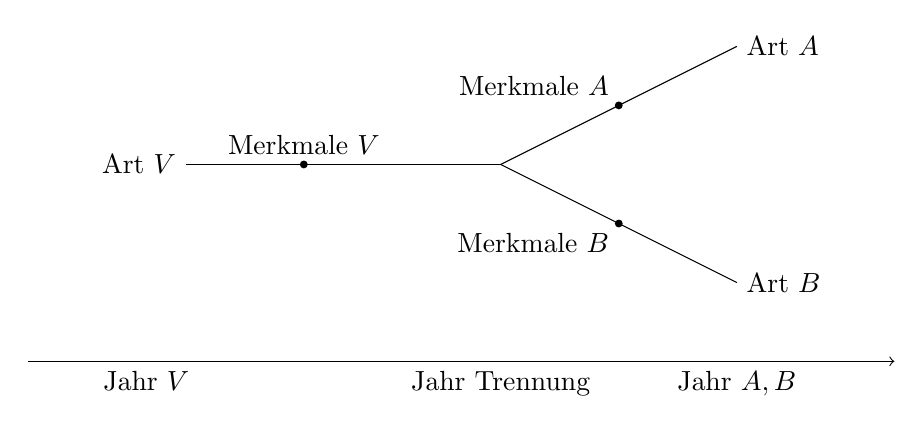
\begin{tikzpicture}
  \node at (0, 0) [left]{Art $V$};
  \fill (1.5, 0) circle (0.05) node[above] {Merkmale $V$};
  \draw (0, 0) -- (4, 0);
  \draw (4, 0) -- (7, 1.5);
  \draw (4, 0) -- (7, -1.5); 
  \fill (5.5, 0.75) circle (0.05) node[above left] {Merkmale $A$};
  \fill (5.5, -0.75) circle (0.05) node[below left] {Merkmale $B$};
  \node at (7, 1.5) [right]{Art $A$};
  \node at (7, -1.5) [right]{Art $B$};
 
  \draw[->] (-2, -2.5) -- (9, -2.5);
  \node at (-0.5, -2.5) [below]{Jahr $V$};
  \node at (4, -2.5) [below]{Jahr Trennung};
  \node at (7, -2.5) [below]{Jahr $A,B$};
 \end{tikzpicture} 
\end{center}
 
\subsection{Mehr Arten} 
Ist beispielsweise eine Tabelle mehrer Arten und dessen Merkmalen gegeben, ist davon auszugehen dass bei jedem Schritt der Evolution nur möglichst wenige Merkmale sich veränderten. Zwei Arten mit ähnlich zur Vorfahren unterschiedlichen Merkmalen gehören in der Regel zusammen auf ein Ast. 
 
Anstelle von phänotypischen Merkmalen kann, für eine genauere Bestimmung, der Genotyp und verwandtes genutzt werden: es kann auch die Aminosäurenkette eines Proteins oder, damit stille Mutationen auch beachtet werden können, direkt die DNA-Sequenz angeguckt werden. Dabei wird jeweils gezählt, wie viele Unterschiede es zwischen den Aminosäurenketten oder den DNA-Basensequenzen der Arten gibt und davon ausgegangen, dass Arten mit weniger Unterschieden evolutionär näher verwandt sind.
\end{document}